%%  **********************************************
%
%   The lines beginning with "%" are comments. 
%   Theses comments explain how to use this template for
%   preparing the MCA Sixth Semester Project Report. 
%
%   The first non-comment line below contains 
%   the matter that go into the preamble of 
%   the input file. These are collected in a 
%   file named "preamble.tex". 
%
%   Do not make any changes in the first 
%   non-comment line below.
%
%%
\documentclass[11pt, oneside, a4paper]{book}
\usepackage{graphicx, fancyhdr, amsmath, times, enumerate, amssymb, calc, multirow, setspace, array}
\usepackage[a4paper,width=150mm,top=35mm,bottom=35mm,bindingoffset=6mm]{geometry}
%% Reference: https://www.overleaf.com/learn/latex/
%% How_to_Write_a_Thesis_in_LaTeX_(Part_2):_Page_Layout
%%
\newcommand{\VAtitle}[1]%
{\def\vtitle{#1}}%
\newcommand{\VAauthor}[1]%
{\def\vauthor{#1}}%
\newcommand{\VAadmissionyear}[1]%
{\def\vadmissionyear{#1}}%
\newcommand{\VAregisternumber}[1]%
{\def\vregisternumber{#1}}%
\newcommand{\VAguide}[1]%
{\def\vguide{#1}}%
\newcommand{\VAhod}[1]%
{\def\vhod{#1}}%
\newcommand{\VAdept}[1]%
{\def\vdept{#1}}%
\newcommand{\VAclass}[1]%
{\def\vclass{#1}}%
\newcommand{\VApaper}[1]%
{\def\vpaper{#1}}%
%%
\linespread{1.3}
\setcounter{secnumdepth}{4}
%%
\usepackage{booktabs}
\usepackage{listings}

%
%   No changes in the next non-comment line.
%
\begin{document}
%
%***************************************************
%
%   No changes in the next comment line.
%
\VApaper{RLMCA352 Project and Viva Voce}%
%
%   In the next line, replace "Report Title" by 
%   the title of your project/thesis.
%
\VAtitle{AUTOMATED TIME TABLE GENERATOR}%
%
%   In the next line, replace "Student" by your name. 
%   Write full name without, repeat without, Mr or Ms
%
\VAauthor{MANJU M KRISHNADAS}%
%
%   In the next line, replace "2016" by the year of  
%   your admission to the College.
%
\VAadmissionyear{2016}%
%
%   In the next line, replace "VExxABCnnn" by your 
%   University Examination Register Number.
%
\VAregisternumber{VAS16MCA34}% 
%
%   In the next line, replace "Guide" by 
%   the full name of your guide or supervisor 
%   with Mr. or Ms. or Dr. or Prof.
%
\VAguide{PROF Aparna S Balan}% 
%
%   No changes in the next three non-comment lines.
%
\VAhod{Dr V N Krishnachandran}
%
\VAdept{Computer Applications}%
%
\VAclass{S6 MCA}%
%
%   The next line is code to print the first few pages: 
%       1. Title page
%       2. Copy of certificate from company
%       3. Certificate from MCA Dept
%       4. Declaration
%       5. Acknowledgment
%   No changes in the next non-comment line.
%
%
%   Redefining plain page style
%  
\fancypagestyle{plain}{%
\fancyhf{} % clear all header and footer fields
\fancyhead[L]{{\small \vtitle}}
\fancyhead[R]{\bf \thepage}
\fancyfoot[C]{\bfseries \thepage} 
\fancyfoot[L]%
{{\scriptsize Department of \vdept, 
Vidya Academy of Science \& Technology, Thrissur}}
\fancyfoot[R]%
{
\includegraphics[width=0.75cm]{VidyaLogo.JPG}}%
\fancyfoot[C]{ }%
\renewcommand{\headrulewidth}{1pt}%
\renewcommand{\footrulewidth}{0.5pt}%
}%
%
\pagestyle{empty}
%
%%
\thispagestyle{empty}
%%
\quad\\[0.5cm]
\begin{center}

\sffamily\small
%
\begin{spacing}{2}
{\fontsize{15.5}{20}\selectfont \bfseries \MakeUppercase{\vtitle}}\\[5cm]
\end{spacing}
%

\begin{spacing}{1.25}
A Project Report submitted by\\[0.25cm]
{\bfseries \vauthor}

{(\vregisternumber)}
\quad\\[0.25cm]
to APJ Abdul Kalam Technological University\\
in partial fulfillment of the requirements for the award of the degree of\\
Master of Computer Applications
\end{spacing}
%
\quad\\[5cm]
%   Logo
%
\includegraphics[width=0.12\textwidth]%
{VidyaLogo.JPG}\\[0.3cm]
%
%   Department particulars
%
\begin{spacing}{1.25}
{\normalsize \sffamily \bfseries Department of \vdept}\\
{\small \sffamily Vidya Academy of Science \& Technology\\ 
\small Thalakkottukara, Thrissur - 680 501}\\
{\sffamily June 2019}
\end{spacing}
%%
\end{center}
%%
%\newpage
%%

%
\pagenumbering{roman}
\newgeometry{left=0.15in, right=0.35in, top=0.35in, bottom=0.25in}
\addcontentsline{toc}{chapter}{Certificate from Company}
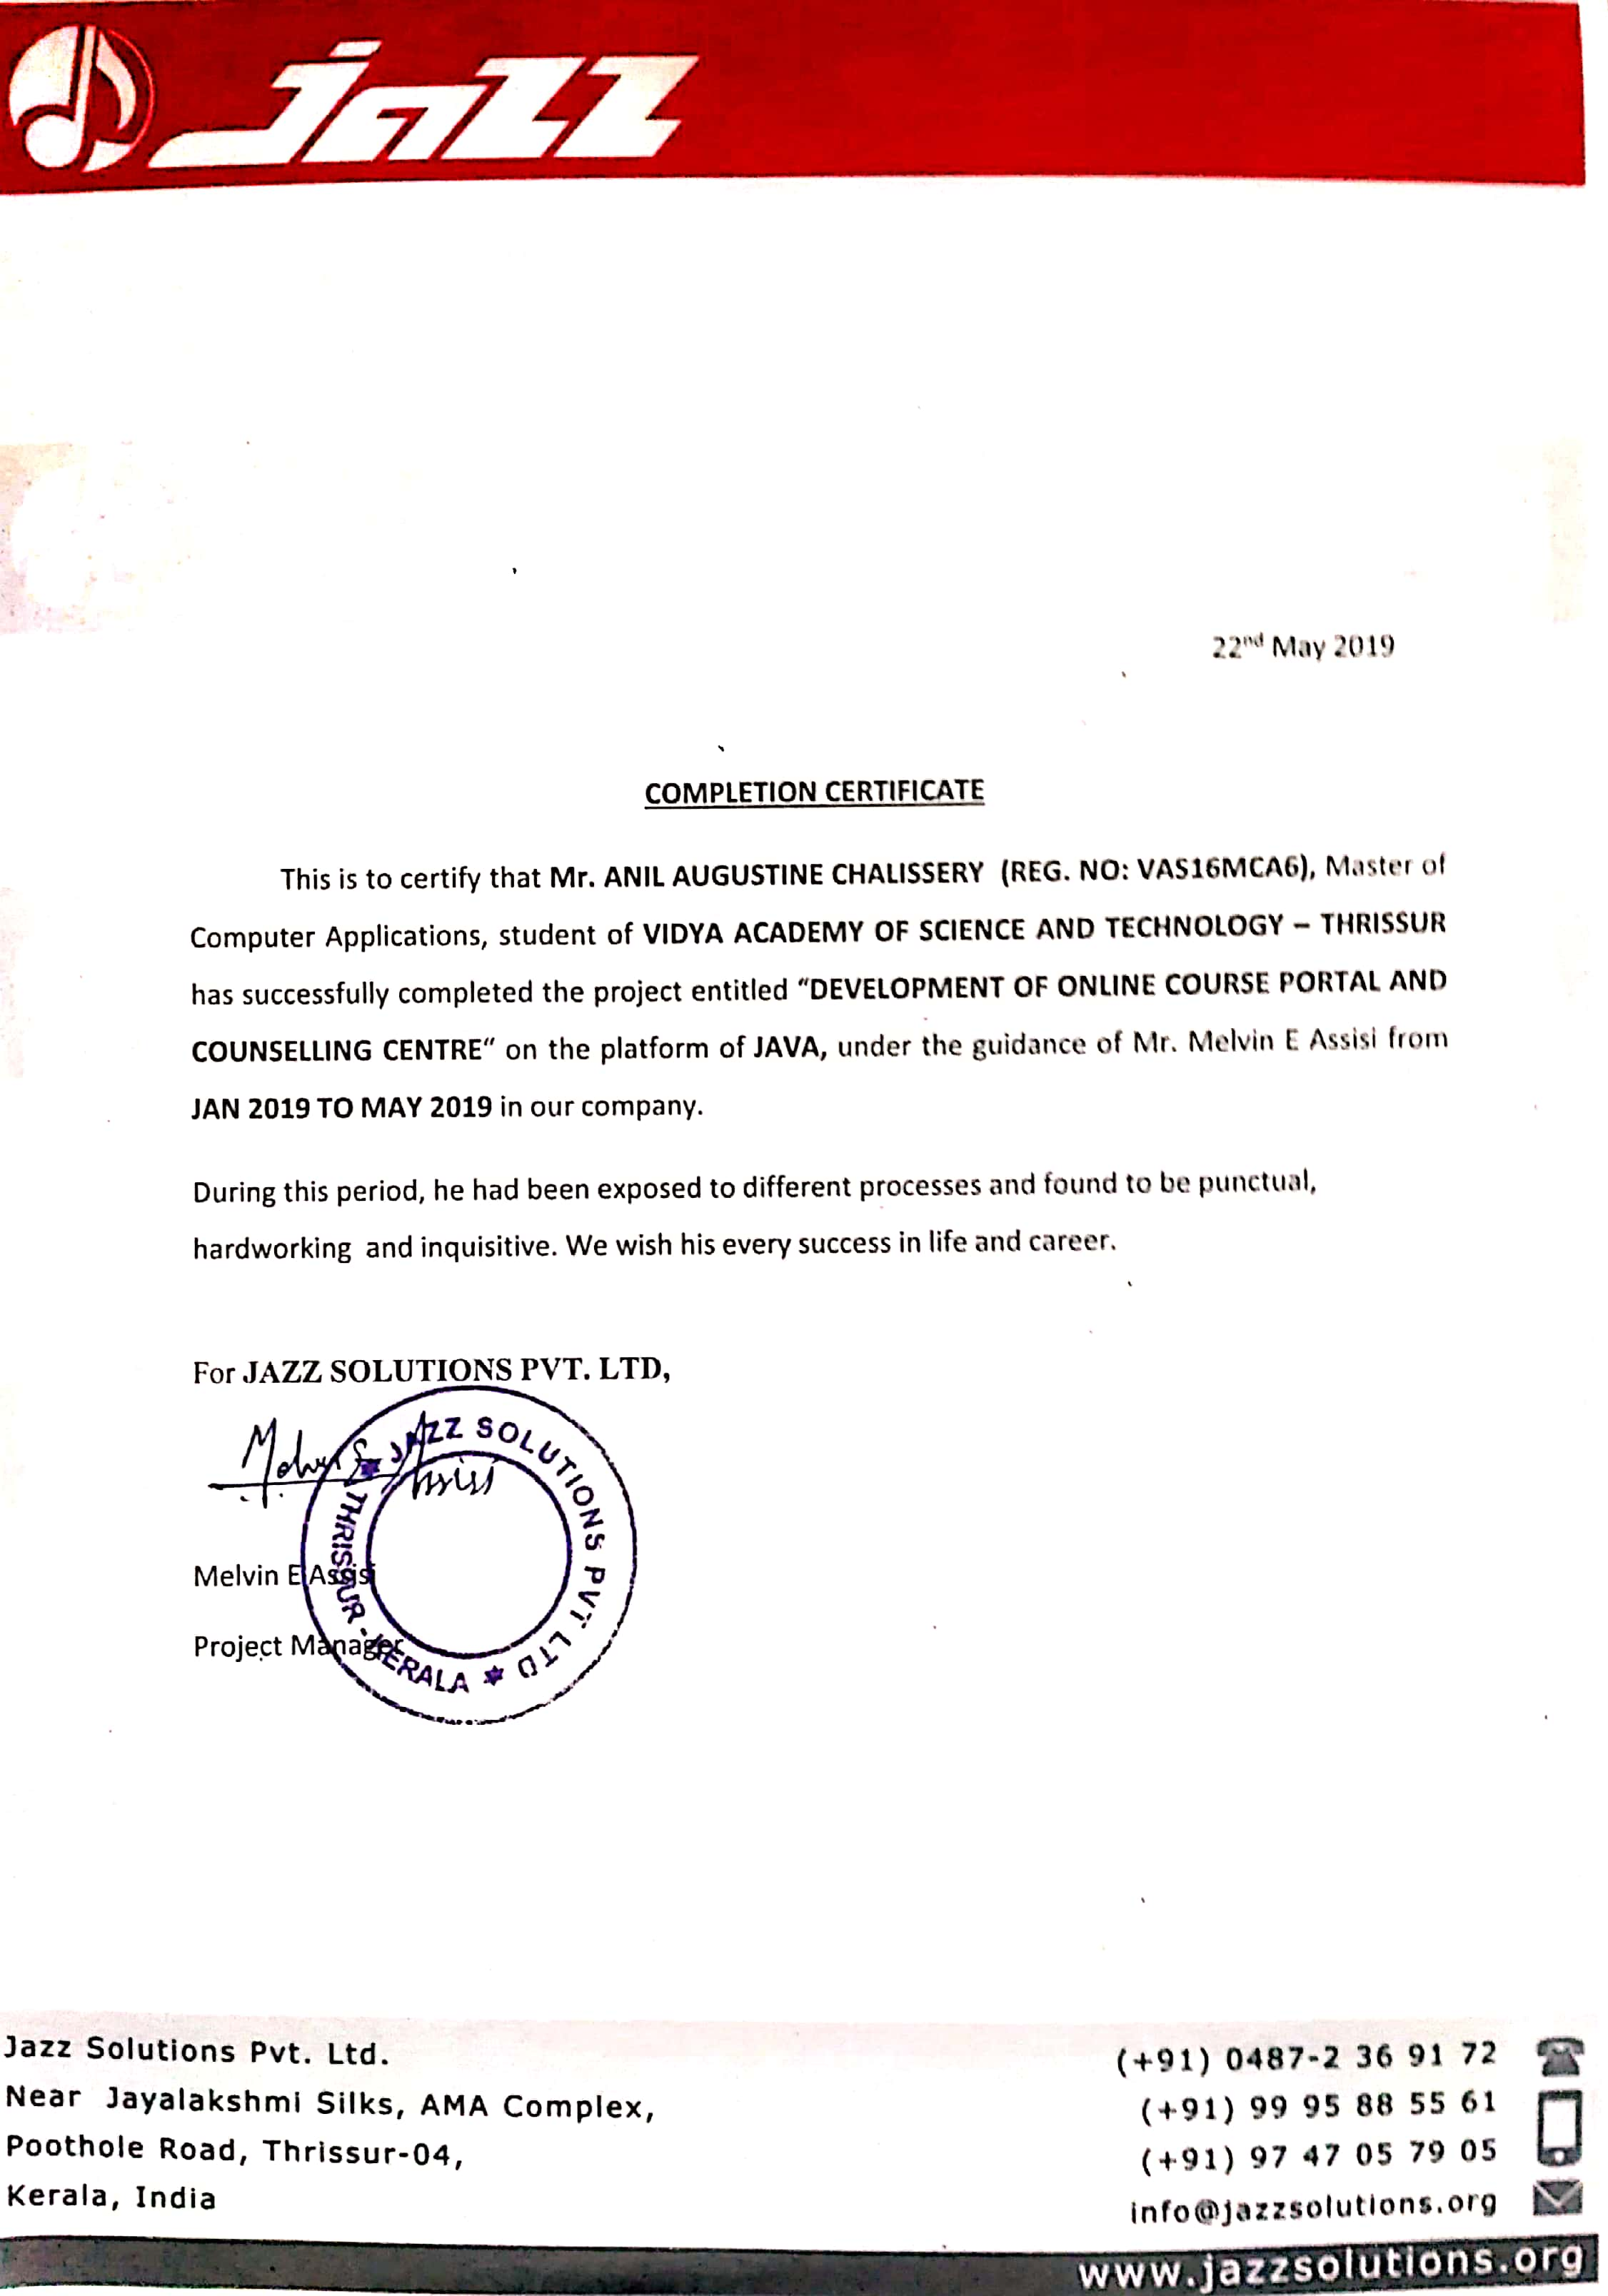
\includegraphics[height=\paperheight-0.75in, width= \paperwidth-0.75in]{certificatee}
\restoregeometry
\newpage
%
\clearpage
%
\addcontentsline{toc}{chapter}{Certificate from College}
%
\vspace*{\fill}
\pagestyle{plain}
\begin{center}
%
%
%   Department particulars
%
{\Large \bf Department of Computer Applications \par  }%\\[0.2cm]
{\large \bf Vidya Academy of Science \& Technology\par}%\\
{\normalsize \bf Thalakkottukara, Thrissur - 680 501\\
({\tt http://www.vidyaacademy.ac.in})\par}
\qquad\\[0.5cm]
%
%   Logo
%

\includegraphics{VidyaLogo.JPG}\\[0.75cm]
%
{\Large \bf CERTIFICATE}\\[0.75cm]
%
\end{center}
%
%   Certificate statement
%
This is to certify that the report titled 
{\bf \vtitle} is a bona-fide record of the 
work related to the paper \vpaper\  done  by 
{\bf \vauthor\  
(Reg. No. \vregisternumber)}    of  \vclass\  
(\vadmissionyear\ admissions) class 
of Vidya Academy of Science \& Technology, 
Thrissur - 680501 in partial fulfillment of the 
requirement for the award of the Degree of Master of Computer Applications  of APJ Abdul Kalam Technological University. \\[0.1cm]
%
%   Spaces for signatures 
%
\begin{center}
\begin{tabular}{p{0.10\textwidth}p{0.35\textwidth}p{0.10\textwidth}p{0.35\textwidth}}
%
\multicolumn{2}{l}{\bf Guide/Supervisor}    
&\multicolumn{2}{l}{\bf Head of Department}   \\
%
Name & : \vguide    & Name & : \vhod \\
%
Signature&: ...........................................
\qquad\quad   & 
Signature&: ...........................................\\
%
Date &: \today    & Date &: \today \\
%
\end{tabular}
\\[0.75cm]
%
%   Space for seal of Department
%
{\small (Seal of Department of \vdept)}
\end{center} 
%
\vspace*{\fill}
%
%   End of Certificate
%  
\clearpage
%
\addcontentsline{toc}{chapter}{Declaration by Student}
\thispagestyle{empty}
\chapter*{Declaration}
%
I, {\bf \vauthor}, studying in Sixth Semester MCA (2016 admissions) class of Vidya Academy of Science \&\  Technology, Thrissur -- 680501,    hereby declare that the project report 
(``\vtitle'') submitted by me for
partial fulfillment of the requirements for the award of degree of Master of Computer Applications of
APJ Abdul Kalam Technological University, Kerala, is a bona fide work done by me
under supervision of \vguide. This submission represents my ideas in
my own words and where ideas or words of others have been included, I have adequately
and accurately cited and referenced the original sources. I also declare that I have
adhered to ethics of academic honesty and integrity and have not misrepresented or
fabricated any data or idea or fact or source in my submission. I understand that any
violation of the above will be a cause for disciplinary action by the institute and/or the
University and can also evoke penal action from the sources which have thus not been
properly cited or from whom proper permission has not been obtained. This report has
not been previously formed the basis for the award of any degree, diploma or similar title
of any other University. 

\qquad\\[1cm]
\begin{tabular}{p{0.05\textwidth}p{0.27\textwidth}p{0.21\textwidth}p{0.35\textwidth}}
%
Place&: Thrissur -- 680501\qquad & Signature of student &: ......................................\\
Date&: \today & Name of student       &: \vauthor
\end{tabular}
\clearpage
%
\addcontentsline{toc}{chapter}{Acknowledgment}
%
\chapter*{Acknowledgment}
%
\index{acknowledgment}
I wish to record my indebtedness and thankfulness 
to all who helped me prepare this Report\index{seminar report} titled 
\vtitle\  and present it in a satisfactory way. This Report is part of my work related to the paper \vpaper.

I am especially thankful to my 
guide and supervisor \vguide\  in the Department of \vdept\  
for giving me valuable suggestions and 
critical inputs in the preparation of this report. 
I am also thankful to \vhod, 
the Head of \vdept\  
for encouragement. 

My friends in my class have always been 
helpful and I am grateful to them for 
patiently listening to  my presentations on my work related  of the project. 

\begin{flushright}
\vauthor\\
Reg. No. \vregisternumber\\
\vclass\  (\vadmissionyear\  Admissions)\\
Vidya Academy of Science \& Technology\\
Thrissur -680 501.
\end{flushright}
%
\clearpage
%
%
%****************************************************
%
%   No changes in the next two non-comment lines. These
%   lines are intended to create the Synopsis page and 
%   to add the the item "Synopsis" to 
%   table of contents.
%
\chapter*{Synopsis}
\addcontentsline{toc}{chapter}{Synopsis}
%
%   Enter below a synopsis of the project report. 
%   The two lines given
%   are to be deleted before entering actual abstract.

          The manual system of preparing timetable in colleges with large number of courses is very time consuming and usually ends up with the same faculty attending more than one class or more than one faculty attending the same class for the same time.


         These are just due to common human errors, which are very difficult to prevent in processes such as these. To overcome these problems people usually taking the previous year’s timetable and modify it, but still it is a tedious job to incoperate changes.


          To overcome all these problems we propose to make an automated system. The system will take various inputs like details of courses, subjects and faculties available, depending upon these inputs it will generate a possible timetable.


        Automated Timetable Generator is a website used to generate timetable automatically.Currently timetable is managed manually. It will help to manage all the periods automatically. It will also manage timetable when any teacher is absent. Here faculties can apply for leave by providing leave required date, reason and also with substitute faculty. Substitute can approve or reject request. Admin can also view the request send by faculty and can view the substitute response. 
	It is a comprehensive timetable management solution for colleges which help to overcome that challenges in mannually setting the timetable. By using this software it will be very easy for faculty to get each and every updates about their periods. 


	This system contains two modules, User Management module and Admin Management module. User Management module can be classified into two, Faculty and Principal.

%
%***************************************************
%
%   The next line creates a Table of Contents. 
%   Do not delete this. There must be a Table of Contents.
%
\clearpage
\addcontentsline{toc}{chapter}{Table of Contents}
\tableofcontents
%
%   The next line creates a page containing a 
%   List of Tables. Delete it if there are no 
%   tables in your project report. 
%
\clearpage
\addcontentsline{toc}{chapter}{List of Tables}
\listoftables
%
%   The next line creates a page containing a 
%   List of Figures. Delete it if there are no 
%   figures in your project report.
%
\clearpage
\addcontentsline{toc}{chapter}{List of Figures}
\listoffigures
%
%***************************************************
%
\mainmatter
%
\clearpage
\quad\vfill
\begin{center}
{\Huge \bf PROJECT REPORT}
\end{center}
\vfill
\clearpage
%
%
%   The main contents of the paper begin here. 
% 
%
%   *********************  CHAPTER ***********************
%
%  
\chapter{INTRODUCTION}
%
\section{Project Overview}

Even though most college administrative work has been computerized, the lecture timetable scheduling is still mostly done manually due to its inherent difficulties. A college timetable is a temporal arrangement of a set of lectures and classrooms in which all given constraints are satisfied. The manual lecture- timetable scheduling demands considerable time and efforts. For example, the same faculty member teaching two courses cannot be assigned to the same time slot. On the other hand, two different courses to be attended by the same group of students also should not clash.


          To overcome all these problems we propose to make an automated system. The system will take various inputs like details of courses, subjects and faculties available, depending upon these inputs it will generate a possible timetable.

               By automating this process with computer assisted timetable generator can save a lot of precious time of administrators, who are involved in creating and managing course timetables. It can easily define faculties adjustments to another class to take up the subject or plays a part of substitution in case of a particular teacher is absent. The aim is here to develop a simple, easily understandable, efficient and portable site which could automatically generate good quality time table with in a second.


                  Automated Timetable Generator is a website used to generate timetable automatically. It will help to manage all the periods automatically. It will also manage timetable when any teacher is absent. Here faculties can apply for leave by providing leave-required date, reason and with substitute faculty. Substitute can approve or reject request.Admin can also view the request send by faculty and can view substitute response.  


		This system contains two modules, User Management module and Admin Management module. User Management module can be classified into two, Faculty and Principal. Each module has it's on duties.

{\bf Admin Module}
\begin{enumerate}
\item Timetable needed to schedule the faculty at provided time slots in such a way that their timings do not overlap. Only the admin can generate timetable for all classes. View timetable class wise and teachers wise.
\item Admin can add the Courses. And possible to view all the courses. Admin can delete the course from the database. And also possible to update the course.
\item Each semester contain different subjects. Only the admin can add subject into the database and admin can update, delete and view the subject details. 
\item Each faculty teaching more than one subjects. Admin can view the all faculties. And admin can update and delete the faculty details. A faculty should have only one class at a time.
\item Admin can also view the substitution request send by faculty and can view substitute response. Alert the substitute and faculty about the substitution details.

\end{enumerate}

{\bf Faculty Module}
\begin{enumerate}
\item Faculties can register their profile itself. At the time a message sent to the registered number of the faculty. Faculties can update their profile. In addition, possible to change the password.
\item Faculties can view the timetable class wise or teacher wise.
\item Faculties can request for substitution by providing leave-required date, reason and with substitute faculty. At the time, a message alert send to the substitute faculty about substitution request.
\item Faculties can view the substitution request send by the faculty. Substitute faculty can accept or reject the substitution request. At the time, response from the substitute faculty sends to the faculty through message alert.
\item Faculties can select subject from various subjects.And view selected subjects.

\end{enumerate}

\newpage
%
\section{Organization Profile}

Allievo Learning Center was established in 2011. Allievo is the training wing of Aumento Performers Solutions Pvt Ltd (An ISO 9001-2008 Certified Company ) with the main objective of promoting IT Education and practices across the Globe.


	It’s a fast growing IT Education Company which has maintained its leadership in imparting quality services. Training programs will help prepare you for employment opportunities through traditional Instructor Led Training, hands-on training, certification achievement, and interviewing preparation. Allievo IT programs designed to give you real-world workplace experience.


	Allievo Learning Center provides the best IT training in the industry, different courses, online training etc. Allievo Learning Center also provide internship, academic project guidance, online training for BTech/BE (ECE, EEE, CSE, IT) , MCA, MSc , MTech, BCA , BSc , Diploma students in different streams like Electronics , Electrical , Computer Science , Information Technology etc.


	Allievo Learning Center provide guideline in different platform like PHP , Android , JAVA ,Embedded System , Digital Image Processing (DIP) , VLSI , NS2 (networking) etc.

We are happy to introduce our self (Allievo Learning Center) as one of the growing training and staffing consultant in Kerala. We provide technical guidance to Software and electronic professionals. We help Professionals and students for specialize their technical skills. We are not just trainers who just provide training and certificate for a technical skill. We make our trainees to suit for the technology.


Allievo Learning Center provide academic project guidance to professional students. Academic project is important section for all kind of professional courses like MTech and Btech. Futuro IT Solutions gives minor and major project guidance to the student of MCA, BTech Computer Science, BTech Electronics, BSC Computer Science, and Diploma students. We will train the technology and make them confident to do their project themselves. That makes them unique in all other Project guidance centers and training institutes in Kerala.


Allievo Learning Center training team is a team of highly talented professionals. They make technical experts rather than professionals. Our hard working team coupled with professionalism results in total efficiency and superior skills, which benefit our clients and trainees alike.


%
%
%   *********************  CHAPTER ***********************
%
%
\chapter{SYSTEM ANALYSIS}

             System Analysis refers to the process of examining a business situation with the intent of improving it through better procedures and methods. System analysis relates to shaping organizations, improving performance and achieving objectives for profitability and growth. The emphasis is on systems in action, the relationships among subsystems and their contribution to meeting a common goal. Looking at a system and determining how adequately it functions, the changes to be made and the quality of the output are parts of system analysis. 
%
\section{The Existing System}	

Planning timetable is one of the most complex and error prone applications. There are still serious problems like high cost generation of time table are occurring while scheduling and these problems are repeating frequently also the difficulty faced during timetabling can be represented as a constraint satisfaction problem with loose parameters and many constraints. In the manual lecture timetabling, one of the major problems is dealing with clashes and finding clash free slots. The same faculty member teaching two courses cannot be assigned the same time slot. Making a change requires that one has to undo previous lecture allocation and look for a new allocations. This creates a series of backtracks which are difficult to resolve.
%< Describe your various components here >
\section{Proposed System}

This project mainly deals with automatically generate timetable. The main users are administrator and faculty. This website helps the admin to generate timetable automatically with maximum avoiding duplication of repeating subjects. Mainly this accounting system consist features like automatically generate timetable and view timetable to faculties. At first they have to add courses and corresponding subjects. After that faculty select subjects. The admin select course and semester then corresponding timetable is generating without duplication. Faculties can apply for leave by providing leave-required date, reason and with substitute faculty. Then selecting a faculty as substitute it allows to view timetable of that faculty for ensure that the faculty is free at that particular period. Substitute can approve or reject request. Admin can also view the request send by faculty and can view substitute response. By automating this process with computer assisted timetable generator can save a lot of precious time of administrators who are involved in creating and managing course timetables.
%
%
%   *********************  CHAPTER ***********************
%
%
\chapter{FEASIBILITY STUDY}

Feasibility study is a test of the system proposal according to its workability, impact on the organization, ability to meet user and effective use of resources. The objective of feasibility study is not to solve the problem. But to acquire a sense of its scope. During this study, the problem definition is crystalized and benefits are estimated with greater detail at this stage. The result of feasibility study is a system formal proposal. This is simply a form of documenting or detailing the nature and scope of proposed solution. The key considerations involved in the feasibility analysis are technical, economic and operational.
%
\section{Technical Feasibility}

This study is performed to check whether the proposed system is technically feasible or not. Any system developed must not have a high demand on the available technical resources. This will lead to high demands on the available technical resources. This will lead to high demands being placed on the client. Technical feasibility centers on the existing computer system (hardware, software, etc) and to what extent it can support the proposed addition. This involves financial consideration to accommodate technical enhancement. This system is technically feasible, all requirements used for this software are reachable. 
%
\section{Economical Feasibility}

This study is the most frequently used method for evaluating the effectiveness of a candidate system. More commonly known as cost/benefit analysis, the procedure is to determine the benefits and savings that are expected from a candidate system and compare them with cost. This analysis phase determines how much cost is needed to produce the proposed system. This system is economically feasible since it does not require any initial setup cost, as the organization has required machines and supporting programs for the application to execute itself. No extra charges are needed for this project.
%
\section{Operational Feasibility}

 This is performed to check whether the system is operationally feasible or not. Using command buttons throughout the application programs enhances operational feasibility. So maintenance and modification is found to be easier. This feasibility is dependent on human resources (software development team) and involves visualizing whether the software will operate after it is developed and be operative once it is installed.A network admin can himself do all things in this system.
%
\chapter{SYSTEM DESIGN }

System designing in terms of software engineering has its own value and importance in the system development process as a whole. To mention it may though seem as simple as anything or simply the design of systems, but in a broader sense it implies a systematic and rigorous approach to design such a system which fulfills all the practical aspects including flexibility, efficiency and security. Systems design is the process of defining the architecture, components, modules, interfaces, and data for a system to satisfy specified requirements. Systems design could be seen as the application of systems theory to product development.

The system design covers the following ,Reviews the current physical system,  Prepares output specifications, Prepares input specifications,  Prepares edit, security and control specifications,  Specifies the implementation plan,  Prepares a logical design walk through of the information flow, output, input, controls  and implementation plan. 


%
\section{Input Design}

The input design is the link between the information system and the user. It comprises the developing specification and procedures for data preparation and those steps are necessary to put transaction data in to a usable form for processing can be achieved by inspecting the computer to read data from a written or printed document or it can occur by having people keying the data directly into the system. The design of input focuses on controlling the amount of input required, controlling the errors, avoiding delay, avoiding extra steps and keeping the process simple. The input is designed in such a way so that it provides security and ease of use with retaining the privacy. Input Design considered the following things that are what data should be given as an input, how the data should be arranged or coded, dialog to guide theoperating personnel in providing input and methods for preparing input validations and steps to follow when error occur.
%
\section{Output Design}

A quality output is one, which meets the requirements of the end user and presents the information clearly. In any system results of processing are communicated to the users and to other system through outputs. In output design it is determined how the information is to be displaced for immediate need and also the hard copy output. It is the most important and direct source information to the user. Efficient and intelligent output design improves the system’s relationship to help user decision-making.

Designing computer output should proceed in an organized, well thought out manner; the right output must be developed while ensuring that each output element is designed so that people will find the system can use easily and effectively. When analysis design computer output, they should Identify the specific output that is needed to meet the requirements.
%
\section{Database Design}

In designing a database application you must set up not only the program‘s routines for maximum performance, but you must pay attention also to the physical layout of the data storage. A good database design does the following:

Provides minimum search times when locating specific records.

Stores the data in efficient manner possible to keep the database from growing too large.

Makes data updates as easy as possible.

It is flexible enough to allow inclusion of new functions required of the program. 
 

 Normalization is a process of converting a relation to a standard form. The process is used to handle the problems that can arise due to data redundancy i.e. repetition of data in the database, maintain data integrity as well as handling problems that can arise due to insertion, updating, deletion anomalies. Insertion anomaly: Inability to add data to the database due to absence of other data. Deletion anomaly: Unintended loss of data due to deletion of other data. Update anomaly: Data inconsistency resulting from data redundancy and partial update. Decomposing is the process of splitting relations into multiple relations to eliminate anomalies and maintain anomalies and maintain data integrity. To do this we use normal forms or rules for structuring relation. Normal Forms are the rules for structuring relations that eliminate anomalies. 
%
%
%   *********************  CHAPTER ***********************
%
%
\chapter{TESTING AND VALIDATION}

In system testing the behavior of whole system or product is tested as defined by the scope of the development project or product. It may include tests based on risks and/or requirement specifications, business process, use cases, or other high level descriptions of system behavior, interactions with the operating systems, and system resources. System testing is most often the final test to verify that the system to be delivered meets the specification and its purpose. System testing is carried out by specialist testers or independent testers. System testing should investigate both functional and non-functional requirements of the testing. 
%
\section{Testing Methods}

{\bf5.1.1. Unit Testing}

 Unit testing is a software testing method by which individual units of source code, sets of one or more computer program modules together with associated control data, usage procedures, and operating procedures, are tested to determine whether they are fit for use. Intuitively, one can view a unit as the smallest testable part of an application. In procedural programming, a unit could be an entire module, but it is more commonly an individual function or procedure. This is one of the main level of testing included in the testing methods. In object-oriented programming, a unit is often an entire interface, such as a class, but could be an individual method. Unit tests are short code fragments created by programmers or occasionally by white box testers during the development process. It forms the basis for component testing. Ideally, each test case is independent from the others. Substitutes such as method stubs, mock objects, fakes, and test harnesses can be used to assist testing a module in isolation. Unit tests are typically written and run by software developers to ensure that code meets its design and behaves as intended. In this system each unit is tested separately before integrating them into modules to test the interfaces between modules. 

{\bf5.1.2. Integration Testing }

When the modules of the system are combined together to form the whole system, there will be the problem of interfacing. Integration testing is a systematic testing technique for constructing the program structure while conducting tests to uncover errors associated with interfacing. The current system modules are combining using bottom-up integration with incremental method. The modules like message, file and watermark are combined to form either embedding or retrieving. Our system, test the integrated modules. In which we test the related forms together to ensure their relationship. 


% < Describe the various Testing methods used here >
\section{Validation}

The definition for the validation testing is that the validation succeeds when software functions in a manner that can be reasonably expected by the customer. The expectations are defined in the software requirements specifications. Validation criteria: The number of characters in the password must contain minimum of four characters. The password will be treated as invalid when the number of characters in it is less than four. Our system, test whether the required fields are empty or not. This system ensure that the fields must be filled and also ensure the minimum range of some fields.

After performing the validation testing, the next step is output testing of the proposed system since no system could be useful if it does not produce the required output in the specific format. The output generated or displayed by the system under consideration is tested asking the users about the format required by then. Here, the output is considered into ways: one is on the screen and the other is printed format. The output format on the screen is found to be correct as the format designed according to the user needs. For the hard copy also, the output comes out as specified by the user. Hence output testing doesn’t result in any connection in the system.
%	< Validation done in the project >
%
%   *********************  CHAPTER ***********************
%
%
\chapter{SYSTEM SECURITY MEASURES}

{\bf Physical }

This site containing the computer systems is physically secured against arms or surreptitious entry by intruders. 

{\bf Operating System }

No matter how to secure the system is, weakness in operating system security may serves as a means of unauthorized access to the network. Here Windows 8.1 as an operating system provides better level of security.  

{\bf Network }

Since almost all network system allows remote access through terminals and networks, software –level security within the network software is important. Network security can be attained by setting firewall and security options available with windows.  

{\bf Database System }

           SQL Server database implementation provides better security to data from unauthorized data access from loss data. SQL Server has built in user management, encryption and restore facility. 


{\bf Correction}

Even with the best quality assurance activities, it is likely that the customer will uncover defects in the software. Corrective maintenance changes the software to correct defects. 

{\bf Password }

 Password is the main security system for our site. This authorization mechanism limits the interaction with the resources to collection of user or system for enforcing integrity, confidentiality or availability constraints. There will be secret password for the user of the system. Hence, authorized users cannot access data of the system.

{\bf Enhancement}

As the software is used, the user will recognize additional functions that will provide benefit. Perfective maintenance extends the software beyond its original functional requirements.


{\bf Adaptation }

Over time, the original environment (e.g. CPU, Operating System, Business Rules, and External Product Characteristics) for which was developed was likely to change. Adaptive maintenance results in the modification to the software to accommodate changes to its external environment.

{\bf System maintenance}

Computer based business systems are dynamic. They must be able to accommodate changes in the business environment. These changes occur not only during the study, design, and development phases of the life cycle of the system, but also throughout its operational life. Maintenance involves the software industry captive, typing up the system resources. It means restoring something to its original condition. Maintenance involves a wide range of activities including correcting, coding and design errors, updating documentation and test data and upgrading user support. Maintenance is continued till the product is re-engineered or deployed to another platform. Maintenance is also done based on fixing the problems reported, changing the interface with other software or hardware enhancing the software.Security measures are provided to prevent unauthorized access of the database at various levels. An uninterrupted power supply should be so that the power failure or voltage fluctuations will not erase the data in the files. 

We can define maintenance by fair different maintenance activities.
\begin {enumerate}
\item Corrective maintenance.
\item Adaptive maintenance.
\item Perfective maintenance or enhancement.
\item Preventive maintenance or reengineering.
\end{enumerate}

{\bf Prevention}

Computer software deteriorates due to change, and because of this, preventive maintenance, often called software reengineering, must be conducted to enable preventive maintenance makes changes to computer programs. So that they can be more easily corrected, adapted and enhanced.

  

%
%
%   *********************  CHAPTER ***********************
%
%
\chapter{CONCLUSION}

The project entitled “AUTOMATIC TIMETABLE GENERATOR” completed successfully in PHP.


                In this Project, I have proposed a mechanism for automated college timetable generation. A college timetable is a temporal arrangement of a set of lectures and classrooms, in which all given constraints are satisfied.The manual lecture- timetable scheduling demands considerable time and efforts. This automated college timetable generator can save a lot of precious time of administrators who are involved in creating and managing course timetables. Automated College Timetable Generator is a website used to generate timetable automatically. The website will make the procedure of time table generation easier consistently.


                Currently timetable is managed manually. Proposed website will help to manage all the periods automatically It will also manage timetable when any teacher is absent.Here faculties can apply for leave by providing leave required date, reason and also with substitute faculty..Substitute can approve or reject substitution request.Admin can also view the request send by faculty and can also view substitute response.

%
\chapter{SCOPE FOR FUTURE ENHANCEMENT}

In future since each and every application should expand and it should provide a way for updating the system has been developed. All modules in the system are being developed carefully. Such that the future enhancement does not affect the basic performance of the system.
\begin{enumerate}
 \item Generate temporary timetable for exam days.
\item Sharing of subject.
\item Alert the students in the case of substitution class.
\item Generation of timetable based on the criteria like
\begin{enumerate}
\item Minimum and maximum workload of each faculty
\item Subject Priority
\end{enumerate}
\end{enumerate}
Later we are also planning to develop this project as an android application. Also extending facility with notifying through SMS can also be applied for future scope.


%
%
%   *********************  CHAPTER ***********************
%
%%%%%%%%%%%%%%%%%%%%%%%%%  APPENDICES %%%%%%%%%%%%%%%%%%%%%
%
\clearpage
\addcontentsline{toc}{chapter}{APPENDICES}
\appendix
\quad\vfill
\begin{center}
{\Huge \bf APPENDICES}
\end{center}
\vfill
\clearpage
%
%
%   *********************  CHAPTER ***********************
%
%
\chapter{SCRUM PROCESS ARTIFACTS}
%
\section{Product Backlog}
%
% The following table is only a sample. 
%
\renewcommand{\arraystretch}{1.25}
\begin{center}
\begin{tabular}{|m{0.08\textwidth}|m{0.15\textwidth}|m{0.5\textwidth}|m{0.1\textwidth}|}
\hline
{\bf Priority} & {\bf Product backlog items} & {\bf User story} & {\bf Estimate (Hours)}\\
\hline
1 & Database creation & As an operations engineer, I want to be able to store all customer information.  & 240 \\
\hline
2 & Login page & As a site member I want to login to the site. & 160 \\
\hline
3 & Category page & As a site member, I want to be able to look for different categories of brands. & 400\\
\hline
4 & Contact page & As a site member, I want to be able to find contact information of the site. & 80 \\
\hline
5 & Banner area & As a marketing personnel, I want to be able to make advertisement. & 40\\
\hline
\end{tabular}
\end{center}
\renewcommand{\arraystretch}{1}
%
%
\subsection{Functional Requirements}

Functional requirements define specific behaviour or functions. A functional requirement describes what a software system should do. The functional requirement is describing the behaviour of the system as it relates to the system's functionality. Here the functional requirements are expressed in terms of each user. Automated college timetable generator contains two types of users. So this project contains two modules. First one is Admin module and second one is Faculty module.

The functional requirement of this project is as follows:

\begin{enumerate}
\item Timetable needed to schedule the faculty at provided time slots in such a way that their timings do not overlap. Only the admin can generate timetable for all classes. View timetable class wise and teachers wise.
\item Admin can add the Courses. And possible to update the course.Admin can delete the course from the database. And also possible to view and update all the courses.
\item Each semester contain different subjects. Only the admin can add subject into the database and admin also can update, delete and view the subject details. 
\item Each faculty teaching more than one subjects. Admin can view the all faculties.And admin can update and delete the faculty details. A faculty should have only one class at a time.
\item Admin can also view the leave request send by faculty and can view substitute response. Alert the substitute and faculty about the substitution status.
\item Faculties can register their profile itself. At the time, a message sent to the registered number of the faculty. Faculties can update their profile. And possible to change the password.
\item Faculties can view the timetable class wise or teacher wise.
\item Faculties can apply for leave by providing leave-required date, reason and with substitute faculty. At the time a message alert send to the substitute faculty about substitution request. Faculties can view the substitution request send by the faculty. Substitute faculty can accept or reject the substitution request. At the time, response from the substitute faculty sends to the faculty through message alert.
\item Faculties can select subject from various subjects. In addition, view selected subjects.

\end{enumerate}

Some properties of a system may be expressed either as a functional or non-functional property. Example The system shall ensure that data is protected from unauthorized access. Conventionally a non-functional requirement (security) because it does not specify specific system functionality expressed as functional requirement: The system shall include a user authorization procedure where users must identify themselves using a login name and password. Only users who are authorized in this way may access the system data. Non-functional requirements may result in new functional requirements statements.

%
\subsection{Non Functional Requirements}

A non-functional requirement is a requirement that specifies criteria that can be used to judge the operation of a system, rather than specific behaviors. Non-functional requirements place constraints on how the system will do so. The non-functional requirement elaborates a performance characteristic of the system. The principal non-functional constraints that is relevant to critical systems: 

\begin{enumerate}
\item Performance

Performance requirements concern the speed of operation of a system. This application provides quick response. Types of performance requirements: 
\begin{enumerate}
\item Response requirements (how quickly the system reacts to a user input) .
\item Throughput requirements (how much the system can accomplish within a specified amount of time) .

\end{enumerate}

\item
 Reliability

Reliability is the ability of a system to perform its required functions under stated conditions for a specific period. This system is reliable because its functionalities can be done on the required conditions. 

\item . Availability 

Availability is the proportion of time a system is in a functioning condition. It refers to the ability of a user to access information or resources in a specified location and in the correct format; this system is available at any time.

\item Security

Security is the degree of resistance to, or protection from, harm. It is the protection of information systems from theft or damage to the hardware, the software, and to the information on them, as well as from disruption or misdirection of the services they provide. 

\item Maintainability 

Maintainability is defined as the probability of performing a successful repair action within a given time. In other words, maintainability measures the ease and speed with which a system can be restored to operational status after a failure occurs.

\item Portability

Portability is the usability of the same software in different environments. It is a characteristic attributed to a computer program if it can be used in operating systems other than the one in which it was created without requiring major rework. 

\end{enumerate}
%
\subsection{System Configuration}

A system configuration (SC) in systems engineering defines the computers, processes, and devices that compose the system and its boundary. More general the system configuration is the specific definition of the elements that define and/or prescribe what a system is composed of.  

Alternatively, the term system configuration can be used to relate to a model. A properly configured system will allow you to avoid nasty resource conflict problems, and make it easier for you to upgrade your system with new equipment in the future. An improperly configured system will lead to strange errors and problems, and make upgrading a big problem.   

%
\subsubsection{Hardware Configuration}

%
\subsubsection{Software Configuration}
%
\subsection{Conceptual Models}

A conceptual model is a model made of the composition of concepts, which are used to help people know, understand, or simulate a subject the model represents.  It is also known as a domain model. Conceptual modelling should not be confused with other modelling disciplines such as data modelling, logical modelling and physical modelling. The conceptual model is explicitly chosen to be independent of design or implementation concerns.   

The aim of a conceptual model is to express the meaning of terms and concepts used by domain experts to discuss the problem, and to find the correct relationships between different concepts. The conceptual model attempts to clarify the meaning of various, usually ambiguous terms, and ensure that problems with different interpretations of the terms and concepts cannot occur. Such differing interpretations could easily cause confusion amongst stakeholders, especially those responsible for designing and implementing a solution, where the conceptual model provides a key artifact of business understanding and clarity. 
%
\subsubsection{ER Diagram/Class Diagram}

         An entity relationship diagram (ERD) shows the relationships of entity sets stored in a database. An entity in this context is a component of data. In other words, ER diagrams illustrate the logical structure of databases. At first glance, an entity relationship diagram looks very much like a flowchart. It is the specialized symbols, and the meanings of those symbols, that make it unique. 

Entities may be characterized not only by relationships, but also by additional properties (attributes), which include identifiers called "primary keys". Diagrams created to represent attributes as well as entities and relationships may be called entity-attribute-relationship diagrams, rather than entity–relationship models.

\begin{figure}[!h]
	\begin{center}
		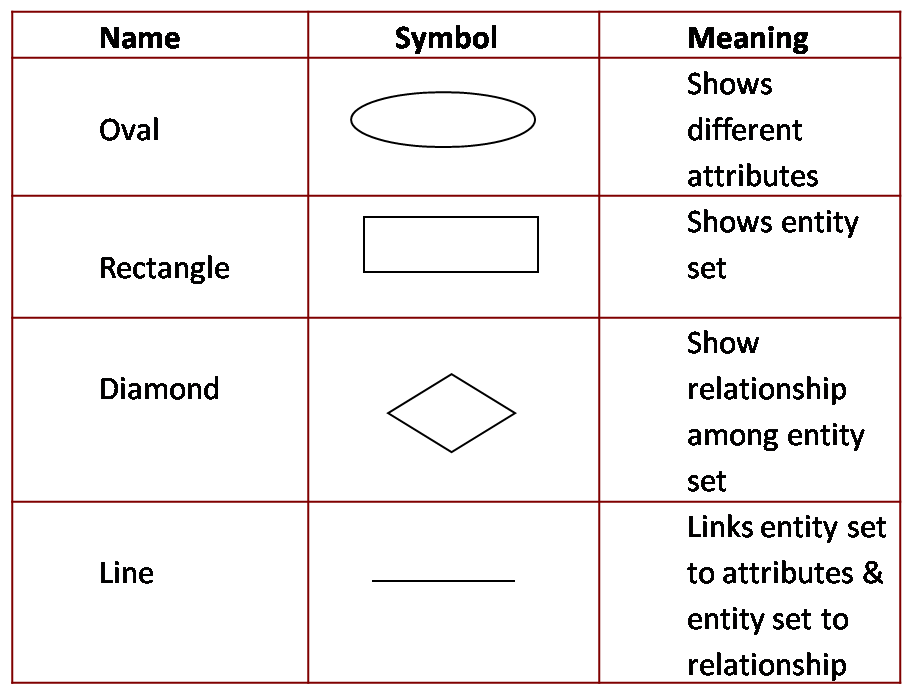
\includegraphics[width=7cm]{ER_Symbol}
	\end{center}
\caption{Symbols Used}
\end{figure}

\begin{figure}[!h]
	\begin{center}
		\includegraphics[height=13cm]{ER_Diagram}
	\end{center}
\caption{ER DIagram}
\end{figure}

%
\subsubsection{Use Case/UML Diagrams}

The use case diagram is used to model the dynamic aspect of the system .A use case diagram shows a set of use cases and actors and their relationships. The use case diagram is mainly used to give an overall view of events that takes place in a trip planning. It specifies flow of events in a trip planning. A use case diagram can be used to view the system‘s functionality from an outside-in perspective and to develop system tests. 

\begin{figure}[!h]
	\begin{center}
		\includegraphics[height=7cm]{UML_Admin}
	\end{center}
\caption{Admin}
\end{figure}

\begin{figure}[!h]
	\begin{center}
		\includegraphics[height=7cm]{UML_Faculty}
	\end{center}
\caption{Faculty}
\end{figure}

\section{Sprint Details}
%
\renewcommand{\arraystretch}{1.25}
\begin{center}
\begin{tabular}{|c|p{4cm}|c|c|c|}
\hline
{\bf Task Name	} & {\bf Description} & {\bf Priority}	& {\bf Status} & {\bf 	Durations (Days)}\\
\hline
Sprint 1 & Requirement Collection and UI Design    &  High     &  Completed  &	 7\\
\hline
Task 1   &	Data Collection  &  High     &  Completed  &  1\\
\hline
Task 2	 & Database Design   &  Medium	&  Completed  &	 2\\
\hline
Task 3	 & UI Design    &  Medium   &  Completed  &	 4\\
\hline
Sprint 2	 & Adding Modules     &  Medium	&  Completed  &  20\\
\hline
Task 1	 & Admin Modules    &  Medium	&  Complete   &  8\\
\hline
Task 2  	 & User Modules	  &  Low	    &  Completed  &  8\\
\hline
Task 3   	& Timetable Management and Validation	  &   Medium	&  Completed  & 4\\
\hline
\end{tabular}
\end{center}
\renewcommand{\arraystretch}{1}
%
\section{Details of daily scrum meeting}
%
Daily scrum meetings were held on each day of a sprint. The meetings were held in the office premises of the team at 9:30 am. These scrum meetings were strictly time-boxed to 15 minutes. This was to keep the discussion brisk but relevant.

All team members were required to attend scrum meetings. Since both the Scrum Master and product owner are committed team members, they are expected to attend and participate. Anyone else was allowed to attend, but was there only to listen. This made scrum meetings an excellent way for a Scrum team to disseminate information.

The daily scrum meeting was not used as a problem-solving or issue resolution meeting. Issues that were raised were taken off-line and usually dealt with by the relevant subgroup immediately after the meeting. During the daily scrum, each team member answered the following three questions:
\begin{itemize}
\item
    What did you do yesterday?
\item
    What will you do today?
\item
    Are there any impediments in your way?
\end{itemize}

By focusing on what each person accomplished on a day and would accomplish the next day, the team would gain an excellent understanding of what work had been done and what work remained. The daily scrum meeting was not a status update meeting in which a boss was collecting information about who was behind schedule. Rather, it was a  meeting in which team members made commitments to each other.
%
\section{Details of bi-weekly meeting}
%
%
\renewcommand{\arraystretch}{1.25}
\begin{center}
\begin{tabular}{|p{2cm}|p{1.5cm}|p{8cm}|}
\hline
{\bf Bi-weekly Meeting No.} & {\bf Date} & {\bf Details} \\
\hline
Bi-weekly Meeting 1 & & Requirement Collection and Database Design \\
\hline
Bi-weekly Meeting 2 & & UI Design  \\
\hline
Bi-weekly Meeting 3 & & Admin Module \\
\hline
Bi-weekly Meeting 4 & & User Module \\
\hline
\end{tabular}
\end{center}
\renewcommand{\arraystretch}{1}
%
%
%   *********************  APPENDIX  ***********************
%
%
\chapter{VERSIONING}
%
%
\renewcommand{\arraystretch}{1.25}
\begin{center}
\begin{tabular}{|p{3cm}|p{5cm}|}
\hline
{\bf Sprint Number} & {\bf Current Version Number}\\
\hline
Sprint 1 & V1.0 \\
\hline
Sprint 2 & V1.1 \\
\hline

\end{tabular}
\end{center}
\renewcommand{\arraystretch}{1}
%
%   *********************  APPENDIX ***********************
%
\chapter{DATA FLOW DIAGRAMS}

Data flow is the one of the best ways of documenting the entire functionality of the system. For the system, which will have some data flows in and have some processing inside and then some data flow out from the system can be documented or represented effectively by means of data flow diagrams. The data flow diagrams are a diagrammatic representation of the system, which has input, process and outputs. Once any system is represented using a data flow diagrams we can identify the following things easily: 
\begin{enumerate}
\item Various entities interacting with the system are identified
\item Flow of data from one entity to another is identified
\item The various processes involved in between the interaction of two or more entities in the system are clearly pointed out.  
\item The various data stores, which hold the data in between the processes, are clearly identified.
\end{enumerate}

\begin{figure}[!h]
	\begin{center}
		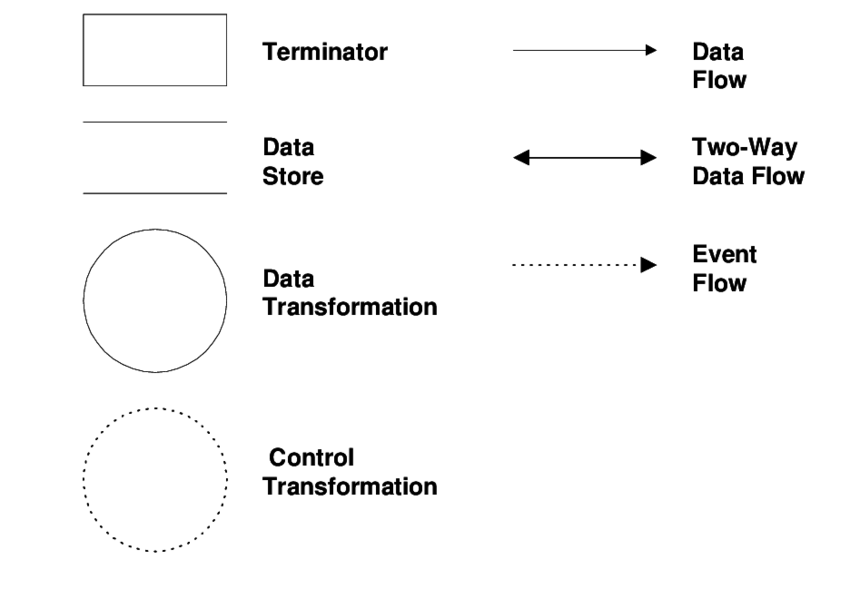
\includegraphics[width=8cm]{DFD_Symbols}
	\end{center}
\caption{DFD Symbols}
\end{figure}


These are various symbols used in the data flow diagrams. Bubbles represent the processes. Named arrows indicate data flow. External entities are represented by rectangles and are outside the system such as vendors and customers with whom the system interacts. They either supply or consume data. Entities supplying data are known as sources and those that consume data are called sinks. Data are stored in a data store by process in the system. Each component in a DFD is labeled with a descriptive name. Process names are further identified with a number. Data flow diagram can be hierarchically organized, which help in partitioning and analyzing large system. As first step, one data flow diagram can depict an entire system, which gives the system overview. It is called Context Diagram or level 0 DFD. The context diagram can be further expanded. The successive expansion of a DFD from the context diagram to those giving more details is known as leveling of DFD. Thus a top down approach is used, starting with an overview and then working out the details.



\begin{figure}[!h]
	\begin{center}
		\includegraphics[width=15cm]{Level_0}
	\end{center}
\caption{Level 0}
\end{figure}

\begin{figure}[!h]
	\begin{center}
		\includegraphics[height=8cm]{Level_1}
	\end{center}
\caption{Level 1}
\end{figure}

\begin{figure}[!h]
	\begin{center}
		\includegraphics[height=9cm]{Level_2}
	\end{center}
\caption{Level 2 - Admin Module}
\end{figure}

\begin{figure}[!h]
	\begin{center}
		\includegraphics[height=9cm]{Level_Faculty}
	\end{center}
\caption{Level 2 - Faculty Module}
\end{figure}

\begin{figure}[!h]
	\begin{center}
		\includegraphics[height=9cm]{Profile_Management}
	\end{center}
\caption{Level 3 - Profile Management}
\end{figure}

\begin{figure}[!h]
	\begin{center}
		\includegraphics[height=9cm]{Subject_Management}
	\end{center}
\caption{Level 3 - Subject Management}
\end{figure}

\begin{figure}[!h]
	\begin{center}
		\includegraphics[height=9cm]{Substitution_Management}
	\end{center}
\caption{Level 3 - Substitution Management}
\end{figure}

\begin{figure}[!h]
	\begin{center}
		\includegraphics[height=9cm]{Timetable_Management}
	\end{center}
\caption{Level 3 - Timetable Management}
\end{figure}



\chapter{TABLE STRUCTURE}
%
%
%   *********************  APPENDIX ***********************
%
\chapter{SAMPLE SCREENSHOTS}


\begin{figure}[!h]
	\begin{center}
		\includegraphics[height=5cm]{home}
	\end{center}
\caption{Home Page}
\end{figure}

\begin{figure}[!h]
	\begin{center}
		\includegraphics[height=5cm]{sign-in}
	\end{center}
\caption{Sign In Page}
\end{figure}

\begin{figure}[!h]
	\begin{center}
		\includegraphics[height=5cm]{admin-home}
	\end{center}
\caption{Admin Dashboard}
\end{figure}

\begin{figure}[!h]
	\begin{center}
		\includegraphics[height=5cm]{admin-course-list}
	\end{center}
\caption{Admin Course List}
\end{figure}

\begin{figure}[!h]
	\begin{center}
		\includegraphics[height=5cm]{admin-set-timetable}
	\end{center}
\caption{Admin Set Timetable}
\end{figure}

\begin{figure}[!h]
	\begin{center}
		\includegraphics[height=5cm]{change-password}
	\end{center}
\caption{Change Password}
\end{figure}

\begin{figure}[!h]
	\begin{center}
		\includegraphics[height=5cm]{user-home}
	\end{center}
\caption{User Home}
\end{figure}

\begin{figure}[!h]
	\begin{center}
		\includegraphics[height=5cm]{user-leave-apply}
	\end{center}
\caption{User Leave Apply}
\end{figure}

\begin{figure}[!h]
	\begin{center}
		\includegraphics[height=5cm]{timetable-view}
	\end{center}
\caption{View Timetable}
\end{figure}

%
%
\clearpage
\addcontentsline{toc}{chapter}{Bibliography}
%
%   The markups for creating the bibliography 
%   begins here. Do not change the two lines 
%   "\begin{thebibliography}{99}" and 
%   "\end{thebibliography}".
%   One sample bibliography item is included. 
%   Each new item is to be preceded by
%   "\bibitem{itemx}".
%   Add additional items if there are any.
%   Bibliography styles:
%   Titles of books   : Italics  {use {\em Title} )
%   URLs of websites  : Type-writer (use {\tt Title} )
%   Titles of papers  : In double quotes (use ``Title")
%
\begin{thebibliography}{99}
%
\bibitem{item1}
{\em First Lessons in \LaTeX}, by Dr. V N Krishnachandran, 
Vidya Academy of Science \& Technology, 
Thrissur - 680 501, 2011.
%
\end{thebibliography}
%
%
%   Printing the last page
%
%
\newpage
\thispagestyle{empty}
\vspace*{\fill}
\begin{flushright}

\includegraphics{VidyaLogo.JPG}\\[0.5cm]
{\Large \bf \sf  Department of \vdept\ }\\
{\sf Vidya Academy of Science \& Technology\\
Thalakkottukara, Thrissur - 680 501\\
({\tt http://www.vidyaacademy.ac.in})}
\end{flushright}
%
%
%
%   ***   The end   ***
%
%
\end{document}